\documentclass[final,3p,times,twocolumn]{elsarticle}
\usepackage[american]{babel}
\usepackage[font=normal]{caption}
\usepackage[font=normal]{subcaption}
\usepackage[tensorialbold]{userCommands}
\usepackage{empheq}
\usepackage{tikz} % geometrical figures
\usetikzlibrary{calc,trees,positioning,arrows,chains,shapes.geometric,decorations.pathreplacing,decorations.pathmorphing,shapes,
    matrix,shapes.symbols,shapes.multipart,patterns,shapes,snakes,pgfplots.groupplots,spy,backgrounds}
\usetikzlibrary{external}
\tikzexternalize[prefix=external/]
\usetikzlibrary{spy,backgrounds}
\usetikzlibrary{decorations.markings}
\usetikzlibrary{arrows.meta}
\tikzset{
  arrows along my path/.style={
    postaction={
      decorate,
      decoration={
        markings,
        mark=between positions 0.03 and 1 step 24pt with {\arrow{Stealth[length=8pt]}},
   }}}}

\usepackage{pgfplots} % pdf picture declaration

\usepackage{array}
\newcolumntype{M}[1]{>{\centering\arraybackslash}m{#1}}
\newcolumntype{N}{@{}m{0pt}@{}}


%% The amssymb package provides various useful mathematical symbols
\usepackage{amssymb}
\usepackage{lineno}
\usepackage{float}
% \linenumbers

\usepackage{float}


\usepackage{mathtools}
\mathtoolsset{showonlyrefs}

\journal{International Journal of Solids and Structures}

\pgfplotsset{%compat=1.3,
  %compat=1.8,
  compat=newest,
  grid=both,
  tick label style={font=\normalsize},
  label style={font=\normalsize},
  legend style={font=\normalsize},
  legend cell align={left},
  yticklabel style={/pgf/number format/fixed},
  %scaled y ticks=false,
  % define user colormap
  colormap={tol}{[1cm] rgb255(0cm)=(120,28,129) rgb255(1cm)=(63,96,174) rgb255(2cm)=(83,158,182) rgb255(3cm)=(109,179,136) rgb255(4cm)=(202,184,67) rgb255(5cm)=(231,133,50) rgb255(6cm)=(217,33,32)}
}

\definecolor{Purple}{RGB}{120,28,129}
\definecolor{Orange}{RGB}{231,133,50}
\definecolor{Blue}{RGB}{63,96,174}
\definecolor{Red}{RGB}{217,33,32}
\definecolor{Duck}{RGB}{83,158,182}
\definecolor{Green}{RGB}{109,179,136}
\definecolor{Yellow}{RGB}{202,184,67}

\newcommand{\review}[1]{\color{Red}#1\color{black}}

\newtheorem{remark}{Remark}


\begin{document}

\begin{frontmatter}


  %% Title, authors and addresses

  %% use the tnoteref command within \title for footnotes;
  %% use the tnotetext command for theassociated footnote;
  %% use the fnref command within \author or \address for footnotes;
  %% use the fntext command for theassociated footnote;
  %% use the corref command within \author for corresponding author footnotes;
  %% use the cortext command for theassociated footnote;
  %% use the ead command for the email address,
  %% and the form \ead[url] for the home page:
  %% \title{Title\tnoteref{label1}}
  %% \tnotetext[label1]{}
  %% \author{Name\corref{cor1}\fnref{label2}}
  %% \ead{email address}
  %% \ead[url]{home page}
  %% \fntext[label2]{}
  %% \cortext[cor1]{}
  %% \address{Address\fnref{label3}}
  %% \fntext[label3]{}
  
  %\title{On the characteristic structure of solutions of hyperbolic systems in two-dimensional elastic-plastic solids.}
  \title{Characteristic structure of wave solutions and resulting loading paths for hyperbolic problems in two-dimensional elastic-plastic solids}
  
  %% use optional labels to link authors explicitly to addresses:
  %% \author[label1,label2]{}
  %% \address[label1]{}
  %% \address[label2]{}
  
  \author{Adrien Renaud$^1$, Thomas Heuz{\'e}, Laurent Stainier}
  
  \address{$^1$ Research Institute in Civil and Mechanical Engineering (GeM, UMR 6183 CNRS)\\
    Ecole Centrale de Nantes \\
    1 rue de la No\"e, Nantes\\
    e-mail: \{adrien.renaud,thomas.heuze,laurent.stainier\}@ec-nantes.fr}
  
  \begin{abstract}
  \end{abstract}
  
  \begin{keyword}
  \end{keyword}


\end{frontmatter}


%% Faire un historique des formulations faites.
%% Formuler le problème à notre sauce et identifier les cas évoqués en intro en particularisant les modules tangents etc. a ce moment, parler des trajets de chargement et des types d'ondes


\section{Introduction}
\label{sec:introduction}
The numerical simulation of physical problems modeled by means of hyperbolic partial differential equations involves the solution of possibly discontinuous waves.
%
The precise tracking of those waves is of major importance in solid mechanics, especially for history-dependent constitutive equations, as it allows to properly assess the residual states.
\review{More specifically, high-speed forming techniques such that electromagnetic forming \cite{Formage} also requires the tracking of solid interfaces.}   
% \note{(a) Examples of applications that involve large deformations}
% \note{Discontinuities + Large deformations!!}
%
Nevertheless, the accurate simulation of such problems can be prevented by several reasons.
%% Mesh-based Lagrangian
First, Lagrangian formulations of mesh-based approaches such as the widely used Finite Element (FEM) \cite{Belytschko} and Finite Volume (FVM) \cite{Leveque} methods become less accurate for very large deformations due to sever distortions of the mesh.
%% Mesh-based Eulerian and ALE
Although those instabilities can be avoided by resorting to Eulerian or Arbitrary Lagrangian-Eulerian formulations, other difficulties arise owing to additional diffusive projections of fields.
%% Time integration
Second, it is well-known that explicit finite element schemes can exhibit numerical noise near sharp solutions that can be hard to remove with artificial viscosity without loss of accuracy.
Such oscillations can nevertheless be removed from FVM solutions due to numerical fluxes involved in the formulation, allowing the building of Total Variation Diminishing (TVD) schemes \cite{Harten}.
%% DG
The Discontinuous Galerkin approximation in space \cite{NeutronDG}, combined with FEM (DGFEM), enables to take advantage of similar interface fluxes so as to construct Total Variation Diminishing in the Means (TVDM) finite element procedures \cite{Cockburn}.
%% Time integration in DGFEM -> STDG
While the introduction of the DG approximation within FEM schemes enables to avoid non-physical oscillations, providing the use of suitable limiters \cite{vanLeer_Limiters}, these approaches are constrained by a restrictive CFL condition \cite{DGFEM_CFL} and hence, suffer from numerical diffusion.
Space-time DGFEM formulations \cite{ST_DGFEM1} enable to circumvent this drawback but are nonetheless subject to mesh entanglement.
%\review{Moreover, the satisfaction of the compatibility condition between reference and updated configurations, through the Piola identity, is not a straightforward undertaking in Lagrangian formulations \cite{Vilar_PiolaIdentity,LagrangianDG_thesis}, which is also the case for finite volumes \cite{Haider_FVM}.
%In other words, updating the geometry based on discontinuous velocities and deformation gradients across element faces may lead to discontinuities in the displacement vector.}


%% MPM
One possibility to avoid mesh tangling instabilities while providing a material description of the motion is to use mesh-free approaches such as those of the Particle-In-Cell (PIC) family \cite{PIC} and, in particular, the Material Point Method \cite{Sulsky94}.
The MPM is based on a dual discretization of a domain made of a collection of material points lying in an arbitrary grid.
A discrete system is solved on the grid, whereas the loading history is stored at particles during the motion so that field projections, which introduce some freedom into the scheme, are required.
%
Indeed, the updated velocity at the grid level can be directly interpolated to the particles according to the original PIC procedure.
Alternatively, the particle velocities can be updated by interpolating the nodal acceleration resulting from the solution of the discrete system, as introduced in PIC by the FLuid Implicit Particle method (FLIP) \cite{FLIP}.
The latter allows to reduce numerical diffusion at the cost of spurious oscillations \cite{PIC_Nishiguchi}.
Recently, a tunable mapping procedure, based on a parameter $m$ that completely eliminates the noise in MPM solutions, has been proposed in the Extended PIC of order $m$ (XPIC(m)) \cite{XPIC}.
A classical interpolation is selected for $m=1$ whereas the mapping tends to FLIP one as $m\rightarrow \infty$.
Nevertheless, the numerical diffusion still prevents from capturing (discontinuous) waves.

%% DGMPM 
\review{
  %A different point of view, which is followed in the Discontinuous Galerkin Material Point Method (DGMPM) \cite{DGMPM,Thesis}, is that the numerical diffusion exhibited by the PIC can be limited by reducing the domain of influence of nodes rather than modifying the projections themselves.
  Note also that the numerical diffusion exhibited by the PIC can be limited by reducing the domain of influence of nodes rather than modifying the projections themselves.
  This approach is followed in the Discontinuous Galerkin Material Point Method (DGMPM) \cite{DGMPM,Thesis}.
  The introduction of the DG approximation within the MPM, combined with the use of the PIC projection, thus aims at providing non-oscillating discontinuous solutions with low numerical diffusion due to the support of the shape functions that reduces to one cell.
  Therefore, the DGMPM enables to take advantage of space-DGFEM and MPM in order to accurately follow waves in finite-deforming media.
}
%
In that method, the weak form of a system of conservation laws is written on an arbitrary grid and numerical fluxes arising from the DG approximation are computed at cell faces by means of an approximate Riemann solver.
Those intercell fluxes allow to take into account the characteristic structure of hyperbolic problems, and in particular the transverse propagation of waves through the use of the Corner Transport Upwind method (CTU) \cite{Colella_CTU} developed for finite volumes.
The CTU is however reformulated in order to fit the DGMPM approximation, in which fields are edge-wise constant in Riemann problems rather than cell-wise constant as it is the case for FVM.
%% Arbitrary grid
Furthermore, as in MPM, all the fields are stored at material points moving in the arbitrary grid, the mapping between nodes and particles being made with PIC projection so that non-oscillating solutions are provided.
\review{Hence, the geometry is updated at the particles level based on a single-valued velocity field. %, in such a way that the difficulties related to the Piola identity are expected to vanish, though it has not been shown so far.
  %% Total Lagrangian
  As a first development step, the DGMPM has been constructed upon a total Lagrangian formulation.
  %
  The numerical results provided by the method for a plane wave problem in a finite-deforming hyperelastic material showed excellent agreement with the exact solution consisting of either a shock or a rarefaction wave \cite{DGMPM}.
  It is worth noticing that similar results can be obtained with the FVM written in the reference configuration, the key point being however that the update of the geometry is straightforward in the DGMPM.
  %
  Furthermore, an interesting feature of the method consists in allowing the employment of mesh adaption strategies so that waves can be accurately captured in the current configuration.
  On the other hand, only linear shape functions leading to a first-order accuracy \cite{Thesis} have been considered, the extension of the method to higher-order approximations being the object of ongoing works.
  The low-order approximation is however not seen as a shortcoming for now since the development of the method has been focused so far on capturing discontinuous solutions for which the accuracy of any numerical scheme falls to one \cite{Leveque}.
}
%Although the equations of solid mechanics are solved in the reference configuration according to a total Lagrangian formulation, an interesting feature of the method consists in allowing the employment of mesh adaption strategies so that waves can be accurately captured in the current configuration.
%% CFL depending on the space discretization
Nonetheless, the stability of the DGMPM highly depends on the distribution of particles inside the computational grid.
Indeed, the stability analysis of the one-dimensional DGMPM scheme coupled to the forward Euler time integration \cite{DGMPM} yields a stability condition that depends on the space discretization and the CFL number.
%
Conversely, one can ensure the stability for a given distribution of material points by finding the CFL number satisfying the aforementioned relation.
%
Such a condition, which does not exist for the MPM and other DGMPM discretizations, is crucial since it allows to: (i) ensure the stability of the scheme while minimizing the numerical diffusion; (ii) adapt the Courant number when the grid is reconstructed; (iii) adapt the grid so that a given CFL condition is satisfied.
It is the purpose of this paper to provide the stability conditions for the one-dimensional DGMPM scheme combined with the two-stage second-order Runge-Kutta (RK2) time discretization and for the two-dimensional DGMPM coupled to the forward Euler algorithm.
\review{
  Although the solution of linear equations is considered here, the results presented must be put into the context of the problems aimed by the method, involving large deformation, and for which the DGMPM enables plenty of perspectives. 
  }

%% Organization of the paper
In the following, the DGMPM discrete system for the multi-dimensional scalar linear advection equation is derived and the computation of interface fluxes, as well as the solution scheme, are recalled in section \ref{sec:dgmpm}.
In particular, we shall see that the adaptation of the Corner Transport Upwind method (CTU) \cite{Colella_CTU} to DGMPM leads to the same corrections of intercell fluxes as for finite volumes.
Second, the system resulting from the combination of DGMPM and RK2 discretization is specialized to one-dimensional problems in section \ref{sec:1d_stab} so that the von Neumann linear stability analysis is carried out.
At last, the same approach is followed in section \ref{sec:2d_stab} for the DGMPM scheme coupled to the forward Euler time integration applied to the two-dimensional problem.


%%% Local Variables:
%%% mode: latex
%%% TeX-master: "manuscript"
%%% End:



\section{Elastic-plastic wave structure in two space dimensions}
\label{sec:charac_plast}
We assume the infinitesimal strain tensor can be additively decomposed into an elastic part and a plastic part according to:
\begin{equation}
  \label{eq:ch5_partition}
  \tens{\eps}=\tens{\eps}^e+\tens{\eps}^p
\end{equation}
The elastic part of the infinitesimal strain tensor is:
\begin{equation}
  \label{eq:ch5_elastic_inverse}
  \tens{\eps}^e = \frac{1+\nu}{E} \tens{\sigma} - \frac{\nu}{E} \tr \tens{\sigma} \tens{I}
\end{equation}

\subsubsection*{The general case}
The governing equations of dynamics in elastic-plastic solids are written in the following quasi-linear form:
\begin{equation}
  \Qcb_t + \Absf^i \drond{\Qcb}{x_i} = \Scb \qquad \text{with: }\Absf^i = -\matrice{\tens{0}^2 & \frac{1}{\rho}\tens{I}\otimes\vect{e}_i\\ \Cbb^{ep}\cdot \vect{e}_i & \tens{0}^4}  \label{eq:ch5_quasilinear}
\end{equation}
where $\Qcb=\matrice{\vect{v}\\ \tens{\sigma}}$ and $\Cbb^{ep}=\ddroit{\tens{\sigma}}{\tens{\eps}}=\Cbb - \beta\tens{m}\otimes\tens{m}$ is the tangent modulus with $\tens{m}=\frac{\tens{s}-\tens{Y}}{\norm{\tens{s}-\tens{Y}}}$ is the flow direction and $\beta=\frac{6\mu^2}{3\mu +(C+R')}$ depends on the shear modulus $\mu$ and kinematic or isotropic hardening modulus $C$ and $R'$ (see section \ref{sec:constitutive-equations}). In particular in the arbitrary direction $\vect{n}$:
\begin{equation}
  \Qcb_t + \Jbsf \drond{\Qcb}{x_n} = \Scb  \label{eq:ch5_quasilinear_normal}
\end{equation}
where $x_n=\vect{x}\cdot\vect{n}$ and the Jacobian matrix $\Jbsf=\Absf^in_i$ arises. The left characteristic fields $\{c_K;\Lcb^K\}$ satisfy the following equation:
\begin{equation}
  \label{eq:ch5_eigen_system}
  \vect{\Lc}^K \(\Jbsf - c_K \Ibsf\) = \vect{0}
\end{equation}
As seen in section \ref{sec:characteristic_analysis}, $6$ couples of characteristic speeds $c_K$ and left eigenvectors $\Lcb^K= \[ \vect{v}^K \: , \: \tens{S}^K \]$ are determined based on those of the acoustic tensor $\tens{A}=\vect{n}\cdot\Cbb^{ep}\cdot \vect{n}$, that are $\{\omega^p;\vect{l}^p\}$ for $p=1,2,3$:
\begin{equation}
  \label{eq:ch5_left_eigenfields}
  \left\lbrace \pm \sqrt{\frac{\omega_p}{\rho_0}} ; \quad \[\: \pm \rho_0\sqrt{\frac{\omega_p}{\rho_0}} \vect{l}^p , -\vect{l}^p\otimes \vect{N} \:\]  \right\rbrace ,\quad p=1,2,3
\end{equation}
In addition, three independent left eigenvectors associated to the zero eigenvalue of system \eqref{eq:ch5_quasilinear_normal}, which is of multiplicity $3$, are found by solving:
\begin{equation}
  \label{eq:ch5_null_eigen}
  \tens{\sigma}^K:\(\Cbb^{ep}\cdot  \vect{n}\) =\vect{0},\quad K=1,2,3
\end{equation}

\subsubsection*{Problems in two space dimensions}
We now focus on the solid domain bounded by $x_1 \times x_2 \times x_3 \in [0,\infty[ \times ]-infty,infty[ \times [-e,e]$ in a Cartesian coordinates system, where $e$ is an arbitrary length.
The solid is subject on the plane $x_1=0$ to a traction force $\vect{T}$ restricted to the $(\vect{e}_1,\vect{e}_2)$ plane, that is $T_3=0$. It is moreover assumed that all quantities except the velocity component $v_3$ depend solely on $x_1$ and $x_2$.

First, the solid is under plane strain, that is $\tens{\eps}\cdot\vect{e}_3=\vect{0}$, if the velocity $v_3$ vanishes on both ends $x_3=\pm h$. Thus, combination of equations \eqref{eq:ch5_partition} and \eqref{eq:ch5_elastic_inverse}, along with the kinematic condition $\eps_{33}=0$, allows to write a relation between $\sigma_{33}$ and other stress components:
\begin{equation}
  \label{eq:plane_strain_stress33}
  \sigma_{33}=\nu\(\sigma_{11}+\sigma_{22}\) - E\eps^p_{33}
\end{equation}

Conversely, if the planes $x_3=\pm e$ are traction free, a plane stress state reading $\tens{\sigma}\cdot\vect{e}_3=\vect{0}$ holds in the solid. For both plane strain and plane stress problems, the stress component $\sigma_{33}$ can then be removed from system \eqref{eq:ch5_quasilinear_normal}, leading to the unknown vector $\Qcb=[v_1,v_2,\sigma_{11},\sigma_{22},\sigma_{12}]$. The problem can then be solved in a two-dimensional setting, for which the acoustic tensor admits two distinct real eigenvalues:
\begin{subequations}
  \begin{alignat}{1}
    \label{eq:ch5_eigenAcc1}
    &\omega_1 = \frac{1}{2}\(A_{11}+A_{22} - \sqrt{(A_{11}-A_{22})^2+4A_{12}}\) \\
    \label{eq:ch5_eigenAcc2}
    &\omega_2 = \frac{1}{2}\(A_{11}+A_{22} + \sqrt{(A_{11}-A_{22})^2+4A_{12}}\) 
  \end{alignat}
\end{subequations}
with associated left eigenvector:
\begin{equation}
  \label{eq:ch5_eigenvectAcc}
  \vect{l}^p=\matrice{-A_{12} \\ A_{11}-\omega_p} = \matrice{ A_{22}-\omega_p \\ -A_{12}}
\end{equation}
From equation \eqref{eq:ch5_left_eigenfields}, one gets that the problem involves two families of waves travelling at speeds $c_1 = \pm \sqrt{\omega_1/\rho}$ and $c_2 = \pm \sqrt{\omega_2/\rho}$. For elastic evolutions, th

that are referred to as \textit{slow} and \textit{fast} waves, travelling respectively at speeds $c_s = \pm \sqrt{\omega_1/\rho}$ and $c_f = \pm \sqrt{\omega_2/\rho}$.
Considering equation \eqref{eq:ch5_left_eigenfields}, the problems involve 









% Orthogonalité des loading paths \cite{Clifton,Ting68}

%%% Local Variables:
%%% mode: latex
%%% TeX-master: "../mainManuscript"
%%% End:


\section{Loading paths through simple waves}
\label{sec:stress_paths}
It has been highlighted that the complete solution of a hyperbolic system in elastic-plastic solids requires to know \textit{a priori} the wave structure.
The object of this section is to study the mathematical properties of the loading functions \eqref{eq:loading_func} in order to get some clues about the stress paths.
It is believed that the information thus earned could be used to accurately approximate the integration of equations \eqref{eq:integral_example}.
First, general properties holding regardless of the loading conditions are highlighted.
Next, the equations are specialized to plane stress and plane strain cases.

\subsection{The general case}
To begin with, let us look at the product of the two loading functions in a direction of space.
Given the left eigenvectors of the acoustic tensor in equation \eqref{eq:eigenvectAcc}, one has for instance:
%Indeed, considering the left eigenvectors of the acoustic tensor given in equation \eqref{eq:eigenvectAcc}, the product $\psi^s_1\psi^f_1$ reads:
\begin{equation*}
  \psi^s_1\psi^f_1 = \frac{l^1_2}{l^1_1}\: \frac{l_2^2}{l^2_1}  
\end{equation*}
Since the eigenvectors of symmetric second-order tensors all satisfy $\vect{l}^1 \cdot \vect{l}^2=0$, it comes out that the above product is equal to $-1$.
Hence, the loading paths resulting from the integration of the ODEs involving $\psi^s_1$ and $\psi^f_1$ are perpendicular in the stress space.
The same goes for $\psi^s_2 $ and $\psi^f_2 $.
Although this orthogonality has already been noticed for particular plane strain and plane stress cases \cite{Clifton,Ting68}, \emph{the generic formulation proposed here shows that this is valid for all problems in two space dimensions}. 
As a result, the study can be restricted to one function in each direction, say $\psi_1^s$ and $\psi_2^s$.


Second, if the function $\psi_1^s$ vanishes at some point of the stress space, the projection in the $(\sigma_{11},\sigma_{12})$ plane of the loading path followed within a slow wave is vertical according to the ODE \eqref{eq:sigSlow_n=e1} (\textit{i.e} $d\sigma_{11}=0$).
Conversely, if $\psi_1^s\rightarrow \infty$, the loading path is horizontal in the $(\sigma_{11},\sigma_{12})$ plane (\textit{i.e} $d\sigma_{12}=0$).
%Looking for vanishing $\psi^f_1$ or $1/\psi^f_1$ amounts to finding roots of the components of $\vect{l}^2$:
These situations respectively correspond to:
\begin{align}
  \label{eq:first_root}
  \psi_1^s = 0  & \Leftrightarrow A_{12} =0  \\
  \label{eq:second_root}
  \psi_1^s \rightarrow \infty & \Leftrightarrow A_{22} -\omega_1 =0
\end{align}
In particular, if $A_{12}=0$ the denominator of $\psi_1^s$ reads:
\begin{equation}
  A_{22} -\omega_1 = \frac{1}{2}\(A_{22} -A_{11} -\sqrt{(A_{11} -A_{22} )^2 + 4A_{12}^2 }\) = \frac{1}{2}\(A_{22} -A_{11} -\abs{A_{11} -A_{22}}\vphantom{\sqrt{(A_{11} -A_{22} )^2 + 4A_{12}^2 }}\) = -\left\langle A _{11}-A _{22}  \right\rangle
\end{equation}
where $\left\langle \bullet \right\rangle=\frac{1}{2}\(\bullet + \abs{\bullet}\)$ denotes the positive part operator.
Therefore, if $A_{12} =0$ and $A_{11} \neq A_{22} $, one has $\psi^s_1 =0$ and hence $\psi^f_1 \rightarrow -\infty $ by orthogonality.
If moreover $A_{11}  = A_{22} $, both components of the eigenvectors vanish and the functions $\psi^s_1$ and $\psi^f_1$ are undetermined.
Note also that in this case, the characteristic speeds of simple waves are identical according to  equations \eqref{eq:eigenAcc1} and \eqref{eq:eigenAcc2}.
  % \begin{equation}
  %   \label{eq:diff_celerities}
  %   \rho c_f^2 - \rho c_s^2 = \sqrt{(A_{11}-A_{22})^2+{4A_{12}}^2} 
  % \end{equation}
  % Then, it follows that the simultaneous satisfaction of conditions \eqref{eq:first_root} and \eqref{eq:second_root} leads to
As a result, the situation $c_f=c_s$ corresponds to a loss of hyperbolicity of the system.

Analogously, the function $\psi_2^s$ is such that:
\begin{align}
    \label{eq:first_root_psi2cp}
    \psi_2^s \rightarrow \infty  & \Leftrightarrow A_{12} =0  \\
    \label{eq:second_root_psi2cp}
    \psi_2^s =0 &  \Leftrightarrow A_{22} -\omega_1 =0
\end{align}
Therefore, if both conditions $A_{12}=0$ and $A_{11} =A_{22}$ are satisfied, the system is no longer hyperbolic with characteristic speeds of fast and slow waves that are identical.

According to the ODEs of table \ref{tab:simpleWavesEquations}, the particular values of the loading functions $\psi_i^{s,f}$ through the simple waves propagating in direction $\vect{e}_i$ for $i=\{1,2\}$, provide information about the loading paths in the stress space.
First, $\psi^{s,f}_i =0$ leads to $d\sigma_{ii}=0$ (no sum on $i$) so that the longitudinal stress is constant within the simple wave.
Conversely, with the loading functions tending to infinity, the stress $\sigma_{12}$ does not vary.
Notice that the coefficients $\alpha_{ij}$ of the left eigenvector of the Jacobian matrix associated with the zero eigenvalue \eqref{eq:null_left_eigen} also have to be regarded.
Nevertheless, those terms resulting from products of the components of the elastoplastic tangent modulus have complex expressions and are assumed to have non-zero values in the remainder of the paper.

The above discussions are now specified to the plane strain and plane stress cases, for which loading conditions leading to $A_{12} =0$ and $A _{11}-A _{22}=0$ are identified.



\subsection{The plane strain case}
The case of plane strain is first considered by using the elastoplastic tangent modulus so that the components of the acoustic tensor for $\vect{n}=\vect{e}_1$ read:
% The elastoplastic tangent modulus under consideration is now that given in equation \eqref{eq:elastoplastic_tangent}, so that the components of the acoustic tensor for $\vect{n}=\vect{e}_1$ read: 
\begin{align}
  \label{eq:DP_A11}
  & A_{11}^{ep}= C_{1111}^{ep} = \lambda + 2\mu -\beta s_{11}^2 \\
  \label{eq:DP_A22}
  & A_{22}^{ep}= C_{2121}^{ep}= \mu -\beta s_{12}^2 \\
  \label{eq:DP_A12}
  & A_{12}^{ep}= C_{1121}^{ep}=-\beta s_{11}s_{12}
\end{align}
The associated eigenvalues are then:
\begin{align}
  \label{eq:eigen_acc_DP1}
  & \rho c_s^2 =  - \frac{\sqrt{\[\lambda + \mu -\beta (s_{11}^2-s_{12}^2) \]^2 +4(\beta s_{11}s_{12})^2}}{2}  
   + \frac{\lambda +3\mu -\beta (s_{11}^2+ s_{12}^2)}{2}
   \\
  \label{eq:eigen_acc_DP2}
  & 
    \rho c_f^2 =    \frac{\sqrt{\[\lambda + \mu -\beta (s_{11}^2-s_{12}^2) \]^2 +4(\beta s_{11}s_{12})^2}}{2}  
     + \frac{\lambda +3\mu -\beta (s_{11}^2+ s_{12}^2)}{2}
\end{align}
Subtracting equations \eqref{eq:DP_A11} and \eqref{eq:DP_A22}, one gets: $A_{11}^{ep}-A_{22}^{ep}= \lambda + \mu -\beta \(s_{11}^2-s_{12}^2\)$.
Hence, the equation $A_{11}^{ep}-A_{22}^{ep}=0$ admits a set of solutions in the deviatoric stress space.
On the other hand, we see from equation \eqref{eq:DP_A12} that $A_{12}^{ep}$ vanishes for $s_{12}=0$ or $s_{11}=0$.
% Recall that $A^{ep}_{12}=0$ leads to vertical and horizontal loading paths across slow and fast waves respectively. 
Each solution is studied in more details below.

%% Sign of one of the functions psi... but not used afterwards
% We first study the sign of the functions $\psi^f$ by noticing that $\mu=\rho c_2^2$ so that $A_{22}^{ep}$ may be rewritten to yield:
% \begin{equation*}
%   \psi^f = -\frac{A_{12}^{ep}}{A_{22}-\rho c_f^2}= -\frac{\beta s_{11}s_{12}}{\rho c_f^2-\rho c_2^2 +\beta s_{12}^2 }
% \end{equation*}
% Since the denominator is positive for $c_f \geq c_2$, it comes out that $\sign (\psi^f) = - \sign(s_{12}) \sign(s_{11})$. Moreover, two roots of the loading function $\psi^f$ can be identified.

%\textbf{Condition $s_{12}=0$}: 
\subsubsection{Condition $s_{12}=0$}
% \review{According to \textsc{Raniecki} \cite[ch.3 p.173]{mandel_book}, this case leads to $c_s =c_2$.}

According to equations \eqref{eq:eigen_acc_DP1} and \eqref{eq:eigen_acc_DP2}, the eigenvalues of the acoustic tensor become:
\begin{align*}
  & \rho c_s^2 = \frac{1}{2}\( \lambda +3\mu -\beta s_{11}^2 - \abs{\lambda + \mu -\beta s_{11}^2 } \) \\
  & \rho c_f^2 = \frac{1}{2}\( \lambda +3\mu -\beta s_{11}^2 + \abs{\lambda + \mu -\beta s_{11}^2 } \)
\end{align*}
Two cases are to be considered:
\begin{itemize}
\item[(i)] if $\beta s_{11}^2 < \lambda + \mu$, the expression further reduces to:
  \begin{align*}
    & \rho c_s^2 = \mu \\
    & \rho c_f^2 = \lambda +2\mu -\beta s_{11}^2 
  \end{align*}
  The characteristic speed of slow waves is therefore equivalent to that of elastic shear waves for plane strain $c_s=c_2=\sqrt{\mu/\rho}$. 
\item[(ii)] if $ \lambda + \mu - \beta s_{11}^2 <0$, the characteristic speeds read: 
  \begin{align*}
    & \rho c_s^2 = \lambda +2\mu -\beta s_{11}^2  \\
    & \rho c_f^2 =  \mu 
  \end{align*}
  Therefore, the celerity of fast waves reduces to that of elastic shear waves.
  Note, however, that the characteristic speed of slow waves remains real if and only if $\lambda +2\mu >\beta s_{11}^2$.
  One then gets the following bounds: $\lambda +2\mu > \beta s_{11}^2 > \lambda +\mu$.
\end{itemize}
Note that the two above situations lead to the propagation of one neutral wave in the medium.
  
At last, the equality $\beta s_{11}^2 = \lambda + \mu$ leads to $A_{11}^{ep}-A_{22}^{ep}=0$ and hence, to undetermined loading functions. 
%% Set of admissible values for s11 (depends on s itself)
% It then appears that the values of $s_{11}$ ensuring hyperbolicity of the system are:
% \begin{equation}
%   s_{11} \in ]-\infty,-\sqrt{\frac{\lambda + \mu}{\beta}}[\: \cup\: ]-\sqrt{\frac{\lambda + \mu}{\beta}},\sqrt{\frac{\lambda + \mu}{\beta}}[\: \cup \:]\sqrt{\frac{\lambda + \mu}{\beta}} ,\infty[
% \end{equation}

%% Discussion about the loading path direction
% Recall that $\psi^f_1$ tending to infinity implies that the loading path are horizontal in $(\sigma_{11},\sigma_{12})$ plane and hence, the fast wave has no influence on the shear stress if, and only if, $\sigma_{12}=0$ downstream.
% Conversely, the stress paths through slow simple waves are vertical.
% Moreover, with regard the last row of table \ref{tab:simpleWavesEquations}, $\sigma_{22}$ is also unchanged in that case.
% As a consequence, if the initial state is shear-free the solution no longer contain combined waves, but longitudinal stress and shear stress simple waves.

% \textbf{Condition $s_{11}=0$}:
\subsubsection{Condition $s_{11}=0$}
Considering the relation \eqref{eq:plane_strain_stress33} between the stress components for plane strain, one writes:
\begin{equation*}
  s_{11}= \frac{2}{3}\sigma_{11}-\frac{1}{3}(\sigma_{22}+\nu(\sigma_{11}+\sigma_{22})-E\eps^p_{33})
\end{equation*}
so that $s_{11}=0$ is equivalent to:
\begin{equation}
  \label{eq:plane_strain_s11=0}
  \sigma_{11}=\frac{1+\nu}{2-\nu}\sigma_{22}-E\eps^p_{33}
\end{equation}
In contrast to what has been seen previously, the functions $\psi^{s,f}$ cannot be undetermined in the case $s_{11}=0$ since the equation $A_{11}^{ep}-A_{22}^{ep}=\lambda + \mu + \beta s_{12}^2=0$ does not admit real solutions.
Nevertheless, the stress state \eqref{eq:plane_strain_s11=0} yields the following characteristic speeds:
\begin{align*}
  & \rho c_s^2 = \mu -\beta s_{12}^2 \\
  & \rho c_f^2 = \lambda +2\mu 
\end{align*}
so that the celerity of fast waves identifies with that of elastic pressure waves under plane strain $c_f=c_1=\sqrt{(\lambda + 2\mu)/\rho}$. %$
Once again, this case corresponds to the propagation of a neutral wave.


%%%% n=e2
$\newline$
The same analysis can be carried out in the direction $\vect{n}=\vect{e}_2$ by considering the following acoustic tensor components:
\begin{align}
  \label{eq:DP_A11_n2}
  & A_{11}^{ep}= C_{1212}^{ep} = \mu -\beta s_{12}^2 \\
  \label{eq:DP_A22_n2}
  & A_{22}^{ep}= C_{2222}^{ep}= \lambda + 2\mu -\beta s_{22}^2 \\
  \label{eq:DP_A12_n2}
  & A_{12}^{ep}= C_{1222}^{ep}=-\beta s_{22}s_{12}
\end{align}
The characteristic speeds are then:
\begin{align}
  \label{eq:eigen_acc_DP1_n2}
  & \rho c_s^2 = - \frac{\sqrt{\[\lambda +\mu -\beta (s_{22}^2-s_{12}^2) \]^2 +4(\beta s_{22}s_{12})^2}}{2} 
    + \frac{\lambda +3\mu -\beta (s_{22}^2+ s_{12}^2)}{2}   
   \\
  \label{eq:eigen_acc_DP2_n2}
  &
      \rho c_f^2 =   \frac{\sqrt{\[\lambda +\mu -\beta (s_{22}^2-s_{12}^2) \]^2 +4(\beta s_{22}s_{12})^2}}{2}
      + \frac{\lambda +3\mu -\beta (s_{22}^2+ s_{12}^2)}{2}   
\end{align}
With these expressions, the same remarks as for $\vect{n}=\vect{e}_1$ can obviously be made by replacing $s_{11}$ with $s_{22}$.

Among the above results, the most significant arises from the condition $s_{12}=0$.
Indeed, it has been seen that $A_{12}^{ep}=0$ leads to $\psi_1^s=0$ and $\psi^s_2\rightarrow \infty$ in such a way that the corresponding loading paths in the $(\sigma_{11},\sigma_{12})$ plane are respectively vertical and horizontal.
Under the orthogonality property of the loading functions, the stress path followed in a fast wave propagating in the direction $\vect{e}_1$ is horizontal in the same plane.
Hence, if the path through a fast wave intersects the plane $\sigma_{12}=0$, the shear stress component remains constant afterwards.
The same result holds for the slow wave propagating in the direction $\vect{e}_2$.
The above conclusion are summarized in table \ref{tab:stress_paths_properties}.
\begin{table*}[h!]
  \centering
  \begin{tabular}{c|ccN}
    \hline
    & \multicolumn{2}{c}{Stress path in ($\sigma_{11},\sigma_{12}$) plane for $\sigma_{12}=0$} &\\ [8pt]
     & $\vect{n}=\vect{e}_1$ ($i=1$)& $\vect{n}=\vect{e}_2$ ($i=2$) &  \\
    \hline
    \hline
    Slow wave: $\ddroit{\sigma_{ii}}{\sigma_{12}}=\psi^s_i \: (i=\{1,2\} \text{ no sum on i})$ & $\psi_1^s=0 \Rightarrow$ vertical path & $\psi_2^s \rightarrow \infty \Rightarrow$ horizontal path &  \\ [15pt]
    Fast wave: $\ddroit{\sigma_{ii}}{\sigma_{12}}=\psi^f_i \: (i=\{1,2\} \text{ no sum on i})$ & $\psi_1^f\rightarrow \infty \Rightarrow$ horizontal path & $\psi_2^f=0 \Rightarrow$ vertical path & \\ [15pt]
    \hline
\end{tabular}
%%% Local Variables:
%%% mode: latex
%%% TeX-master: "../manuscript"
%%% End:

  \caption{Loading paths projected on the ($\sigma_{11},\sigma_{12}$) plane followed across slow and fast simple waves, under the condition $\sigma_{12}=0$ assuming that $A_{11}^{ep}-A_{22}^{ep}\neq 0$.}
  \label{tab:stress_paths_properties}
\end{table*}
\subsection{The plane stress case}
% The elastoplastic tangent modulus under consideration is now that given in equation \eqref{eq:CP_constitutive}.
As mentioned in section \ref{sec:2dproblem}, a suitable elastoplastic tangent modulus $\widetilde{\Cbb}^{ep}$ is now under consideration.
Let's first focus on $\psi_1^s$ related to the vector $\vect{n}=\vect{e}_1$.
Thus:
\begin{align}
  \label{eq:CP_A11}
  &
      \widetilde{A}_{11}^{ep}= \: C^{ep}_{1111} - \frac{(C^{ep}_{1133})^2}{C^{ep}_{3333}} =\:\lambda + 2\mu -\beta s_{11}^2 -\frac{\(\lambda -\beta s_{11}s_{33}\)^2}{\lambda + 2\mu - \beta s_{33}^2}  \\
  \label{eq:CP_A22}
  &
      \widetilde{A}_{22}^{ep}=  \: C^{ep}_{2121} - \frac{(C^{ep}_{2133})^2}{C^{ep}_{3333}} =\:\mu - \beta s_{12}^2 -\frac{\(\beta s_{12}s_{33}\)^2}{\lambda + 2\mu - \beta s_{33}^2}   
\\
  \label{eq:CP_A12}
  &
      \widetilde{A}_{12}^{ep} = \: C^{ep}_{1121} - \frac{C^{ep}_{1133}C^{ep}_{1233}}{C^{ep}_{3333}} =\:\beta s_{12} \frac{\lambda s_{33} - (\lambda + 2\mu)s_{11} }{\lambda + 2\mu - \beta s_{33}^2}
\end{align}
In order to ensure the hyperbolicity of the system, the components of the acoustic tensor also have to be defined, that is $C^{ep}_{3333}> 0$, which leads to:
\begin{equation*}
  \lambda + 2\mu - \beta s_{33}^2 > 0 \quad \Leftrightarrow \quad s_{33}^2 < \frac{\lambda + 2\mu}{\beta}
\end{equation*}
Second, from equation \eqref{eq:CP_A12}, $\widetilde{A}_{12}^{ep}$ admits two roots in terms of the components of the deviatoric stress tensor, namely: 
\begin{equation}
  s_{12}=0 \quad ; \quad s_{11}= \frac{\lambda}{\lambda+2\mu}s_{33}
\end{equation}
In terms of the components of the Cauchy stress tensor, these conditions read:
\begin{equation}
  \label{eq:CP_roots}
  \sigma_{12}=0 \quad ; \quad \sigma_{11}=\frac{2\mu}{3\lambda+4\mu}\sigma_{22}
\end{equation}
% Hence, the loading path through a slow simple wave is vertical, that is $\psi^s_1 = 0$, for stress values satisfying \eqref{eq:CP_roots}, providing that the $\widetilde{A}_{11}^{ep}$ and $\widetilde{A}_{22}^{ep}$ are not equal.
% Conversely, such stress states yield horizontal path through a fast wave.


% \textbf{Case $s_{12}=0$ :}
% \begin{align}
%   & \rho c_s^2 =\frac{1}{2}\(\widetilde{A}_{11}^{ep}+\widetilde{A}_{22}^{ep} - \abs{\widetilde{A}_{11}^{ep}-\widetilde{A}_{22}^{ep}}\) \\
%   & \rho c_f^2 =\frac{1}{2}\(\widetilde{A}_{11}^{ep}+\widetilde{A}_{22}^{ep} + \abs{\widetilde{A}_{11}^{ep}-\widetilde{A}_{22}^{ep}}\)
% \end{align}

If on the other hand the vector $\vect{n}=\vect{e}_2$ is considered, the acoustic tensor components read:
\begin{align}
    \label{eq:CP_A11_n=e2}
    & \widetilde{A}_{11}^{ep}= C^{ep}_{1212} - \frac{(C^{ep}_{1233})^2}{C^{ep}_{3333}} = \mu -\beta s_{12}^2 -\frac{\(\lambda -\beta s_{12}s_{33}\)^2}{\lambda + 2\mu - \beta s_{33}^2} \\
    \label{eq:CP_A22_n=e2}
    & \widetilde{A}_{22}^{ep}= C^{ep}_{2222} - \frac{(C^{ep}_{2233})^2}{C^{ep}_{3333}}= \lambda +2\mu - \beta s_{22}^2 -\frac{\(\beta s_{22}s_{33}\)^2}{\lambda + 2\mu - \beta s_{33}^2} \\
    \label{eq:CP_A12_n=e2}
    & \widetilde{A}_{12}^{ep} = C^{ep}_{1222} - \frac{C^{ep}_{1233}C^{ep}_{2233}}{C^{ep}_{3333}} =\beta s_{12} \frac{\lambda s_{33} - (\lambda + 2\mu)s_{22} }{\lambda + 2\mu - \beta s_{33}^2}
    %     \label{eq:CP_A11_n=e2}
    % & \widetilde{A}_{11}^{ep}=  \mu -\beta s_{12}^2 -\frac{\(\lambda -\beta s_{12}s_{33}\)^2}{\lambda + 2\mu - \beta s_{33}^2} \\
    % \label{eq:CP_A22_n=e2}
    % & \widetilde{A}_{22}^{ep}= \lambda +2\mu - \beta s_{22}^2 -\frac{\(\beta s_{22}s_{33}\)^2}{\lambda + 2\mu - \beta s_{33}^2} \\
    % \label{eq:CP_A12_n=e2}
    % & \widetilde{A}_{12}^{ep} = \beta s_{12} \frac{\lambda s_{33} - (\lambda + 2\mu)s_{22} }{\lambda + 2\mu - \beta s_{33}^2}
\end{align}
These expressions are similar to those obtained before with $s_{22}$ instead of $s_{11}$.
It comes out that $\widetilde{A}_{12}^{ep}$ admits two roots in the case $\vect{n}=\vect{e}_2$:
\begin{equation}
  \label{eq:CP_roots_n=e2}
  \sigma_{12}=0 \quad ; \quad \sigma_{22}=\frac{2\mu}{3\lambda+4\mu}\sigma_{11}
\end{equation}

The complexity introduced by the plane stress tangent modulus prevents finding other singular configurations for the hyperbolic system. 
In particular, it is difficult to deal with the equation $\widetilde{A}^{ep}_{11}=\widetilde{A}^{ep}_{22}$ due to the expressions given in equations \eqref{eq:CP_A11} and \eqref{eq:CP_A22}.
Nevertheless, since the stress state $s_{12}=0$ also constitutes a singular point for plane stress, the same remarks as those made for the plane strain loading path hold.
Namely, $\sigma_{12}$ becomes constant if it falls to zero along the loading path followed inside a fast (\textit{resp. slow}) wave propagating in direction $\vect{e}_1$ (\textit{resp. $\vect{e}_2$}), as summarized in table \ref{tab:stress_paths_properties}.
%Namely, if $\sigma_{12}$ falls to zero along the loading path followed inside a fast (\textit{resp. slow}) wave propagating in direction $\vect{e}_1$ (\textit{resp. $\vect{e}_2$}), is restricted to that value.
%As we shall see below, more singular behaviors can be identified for plane strain.



%%% Local Variables:
%%% mode: latex
%%% TeX-master: "manuscript"
%%% End:



\section{Numerical integration of stress paths}
\label{sec:numerical_results}
The DGMPM is now illustrated on numerical examples considering materials based on the Hencky-based hyperelastic-plastic potential presented in \cite{Laurent2009} and isotropic hardening. 
The values of material parameters used are gathered in table \ref{tab:material}, the elastic behavior being given by Young's modulus $E$ and Poisson's ratio $\nu$, and plastic flow governed by the yield stress in tension $\sigma^y$ and the hardening coefficient $H$.
\begin{table}[h!]
  \centering
    \begin{tabular}{l|lN}
    \hline
    $E=2\times 10^{11}\:Pa$ & $\sigma^y=1 \times 10^8 Pa$ & \\ [3pt]
    $\nu=0.3$ & $C=10^{8} Pa$  &\\[3pt]
    $\rho_0 = 7800 \: kg.m^{-3}$ & &\\[3pt]
    \hline
  \end{tabular}

%%% Local Variables:
%%% mode: latex
%%% TeX-master: "../manuscript"
%%% End:

  \caption{Material parameters.}
  \label{tab:material}
\end{table}

\subsection{Plane wave problem}
\label{sec:plane-wave-problem}
Let's first look at the response of a infinite medium in directions $\vect{e}_2$ and $\vect{e}_3$ and length $l=1\:m$ in direction $\vect{e}_1$, to Riemann-type initial conditions on the velocity: $v_1=v_d>0$ for $X\in[0,l/2[$ and $v_1=-v_d$ for $X \in ]l/2,l]$.
The solid is initially in a free stress state and the initial velocity is set so that plastic flow occurs:
\begin{equation*}
  v_d=1.2\frac{Y_H}{\rho c_L}
\end{equation*}
where $Y_H=(\lambda+2\mu)\sigma^y/2\mu$ denotes the Hugoniot elastic limit, $c_L=\sqrt{(\lambda+2\mu)/\rho}$ is the elastic pressure wave speed, and $(\lambda,\mu)$ are Lam\'e's constants. Both ends of the medium are traction free.
%so that rightward and leftward compressive elastic waves reflect as unloading waves that interact with the incident plastic ones \cite{Thomas_EVP}.
The initial setting is assumed to give rise to a plane wave, namely:
\begin{align*}
  & \tens{F}= F \vect{e}_1 \otimes\vect{e}_1 + \vect{e}_2 \otimes\vect{e}_2 + \vect{e}_3 \otimes\vect{e}_3\\
  & \tens{\Pi}=\Pi_L \vect{e}_1 \otimes \vect{e}_1 + \Pi_T \(\vect{e}_2 \otimes \vect{e}_2+\vect{e}_3 \otimes \vect{e}_3\) 
\end{align*}
In the linearized geometrical limit $\norm{\tens{F}} \ll 1$ and considering linear isotropic hardening, the computed hyperelastic-plastic solution should tend to the elastoplastic one derived in \cite{Thomas_EP}.
The latter consists of two elastic compression waves propagating left and right-ward, each followed by one plastic discontinuity.
The incident elastic disturbances then reflect as unloading waves on both free boundaries of the domain, the interaction of which at the center of the medium leads to tensile plastic reloading.
In figure \ref{fig:hep_planeWave}, the numerical solutions provided by the DGMPM, the MPM and the FEM are compared to the exact solution of the small strain problem in terms of longitudinal components of the PK1 stress and the Green-Lagrange plastic strain $\tens{E}^p=\frac{1}{2}\({\tens{F}^p}^T\tens{F}^p - \tens{I}\)$.
Linear elements and a lumped mass matrix are used within FEM with no artificial viscosity added, and mesh is built so that Gauss' points are consistent with the particles.
Moreover, while the MPM is only based on a one-particle-per-cell (1ppc) space discretization, DGMPM computations have also been done with two-particles-per-cell (2ppc).
In the latter case, the material points sharing an element are placed symmetrically with respect to elements centers and are regularly spaced in the domain.
For the comparison, all numerical methods are based on a total Lagrangian formulation and make use of the same variational constitutive update.
\begin{figure}[ht]
  \centering
  {\phantomsubcaption{\label{subfig:he_planeWave1}}}
  {\phantomsubcaption{\label{subfig:he_planeWave2}}}
  {\phantomsubcaption{\label{subfig:he_planeWave3}}}
  \begin{tikzpicture}[spy using outlines={rectangle, magnification=3, size=1.cm, connect spies},scale=.8]
  \begin{groupplot}[group style={group size=3 by 2,ylabels at=edge left, yticklabels at=edge left,horizontal sep=2.ex,vertical sep=4ex,xticklabels at=edge bottom,xlabels at=edge bottom},ymajorgrids=true,xmajorgrids=true,enlargelimits=0,xmin=0.5,xmax=1.,xlabel=$x (m)$,axis on top,scale only axis,width=0.33\linewidth,height=0.25\linewidth]

    % ============================== Stress Line
    % t1 % t= 6.84e-5
    \nextgroupplot[title={(a) $t = 6.84\times 10^{-5} $ s.},ylabel=$\Pi_L \: (Pa)$,ymin=-8.5e8,ymax=8.e8]
    \addplot[Red,densely dashed,thick] table[x=x,y=Pi] {pgfFigures/HEP_planeWave/mpm0.pgf};
    \addplot[Green,densely dotted,very thick] table[x=x,y=Pi] {pgfFigures/HEP_planeWave/mpm_2ppc0.pgf};
    \addplot[Blue,mark=asterisk,thick,mark repeat=2,mark size=3pt] table[x=x,y=Pi] {pgfFigures/HEP_planeWave/dgmpm0.pgf};
    \addplot[Purple,mark=x,thick,mark repeat=2,mark size=3pt] table[x=x,y=Pi] {pgfFigures/HEP_planeWave/dgmpm_2ppc0.pgf};
    \addplot[Orange,mark=*,thick,mark repeat=2,mark size=2pt] table[x=x,y=Pi] {pgfFigures/HEP_planeWave/fem0.pgf};
    \addplot[black] table[x=x,y=Pi] {pgfFigures/HEP_planeWave/exact0.pgf};

    % \begin{scope}
    %   \spy[black,size=2.cm] on (3.7,0.35) in node [fill=none] at (2.725,3.);
    % \end{scope}

    % t2 % t= 1.37e-4
    \nextgroupplot[title={(b) $t=1.37\times 10^{-4}$ s.},ymin=-8.5e8,ymax=8.e8]
    \addplot[Red,densely dashed,thick] table[x=x,y=Pi] {pgfFigures/HEP_planeWave/mpm1.pgf};
    \addplot[Green,densely dotted,very thick] table[x=x,y=Pi] {pgfFigures/HEP_planeWave/mpm_2ppc1.pgf};
    \addplot[Blue,mark=asterisk,thick,mark repeat=2,mark size=3pt] table[x=x,y=Pi] {pgfFigures/HEP_planeWave/dgmpm1.pgf};
    \addplot[Purple,mark=x,thick,mark repeat=2,mark size=3pt] table[x=x,y=Pi] {pgfFigures/HEP_planeWave/dgmpm_2ppc1.pgf};
    \addplot[Orange,mark=*,thick,mark repeat=2,mark size=2pt] table[x=x,y=Pi] {pgfFigures/HEP_planeWave/fem1.pgf};
    \addplot[black] table[x=x,y=Pi] {pgfFigures/HEP_planeWave/exact1.pgf};

    % t3 % t= 2.05e-4
    \nextgroupplot[title={(c) $t=2.05\times 10^{-4}$ s.},ymin=-8.5e8,ymax=8.e8]
    \addplot[Red,densely dashed,thick] table[x=x,y=Pi] {pgfFigures/HEP_planeWave/mpm2.pgf};
    \addplot[Green,densely dotted,very thick] table[x=x,y=Pi] {pgfFigures/HEP_planeWave/mpm_2ppc2.pgf};
    \addplot[Blue,mark=asterisk,thick,mark repeat=2,mark size=3pt] table[x=x,y=Pi] {pgfFigures/HEP_planeWave/dgmpm2.pgf};
    \addplot[Purple,mark=x,thick,mark repeat=2,mark size=3pt] table[x=x,y=Pi] {pgfFigures/HEP_planeWave/dgmpm_2ppc2.pgf};
    \addplot[Orange,mark=*,thick,mark repeat=2,mark size=2pt] table[x=x,y=Pi] {pgfFigures/HEP_planeWave/fem2.pgf};
    \addplot[black] table[x=x,y=Pi] {pgfFigures/HEP_planeWave/exact2.pgf};
    
    % \begin{scope}
    %   \spy[black,size=1.5cm] on (9.65+2.,3.5) in node [fill=none] at (11+3.2,1.25);
    % \end{scope}

    % ============================== Plastic strain Line
    % t1
    \nextgroupplot[ylabel=$E^p_{11}$,ymin=-1.12e-3,ymax=2.e-4]
    \addplot[Red,densely dashed,thick] table[x=x,y=epls] {pgfFigures/HEP_planeWave/mpm0.pgf};
    \addplot[Green,densely dotted,very thick] table[x=x,y=epls] {pgfFigures/HEP_planeWave/mpm_2ppc0.pgf};
    \addplot[Blue,mark=asterisk,thick,mark repeat=2,mark size=3pt] table[x=x,y=epls] {pgfFigures/HEP_planeWave/dgmpm0.pgf};
    \addplot[Purple,mark=x,thick,mark repeat=2,mark size=3pt] table[x=x,y=epls] {pgfFigures/HEP_planeWave/dgmpm_2ppc0.pgf};
    \addplot[Orange,mark=*,thick,mark repeat=2,mark size=2pt] table[x=x,y=epls] {pgfFigures/HEP_planeWave/fem0.pgf};
    \addplot[black] table[x=x,y=epls] {pgfFigures/HEP_planeWave/exact0.pgf};
    
    % t2
    \nextgroupplot[legend style={at={($(0.9,-0.45)+(2.1cm,0.65cm)$)},legend columns=3},ymin=-1.12e-3,ymax=2.e-4]
    \addplot[Red,densely dashed,thick] table[x=x,y=epls] {pgfFigures/HEP_planeWave/mpm1.pgf};
    \addplot[Green,densely dotted,very thick] table[x=x,y=epls] {pgfFigures/HEP_planeWave/mpm_2ppc1.pgf};
    \addplot[Blue,mark=asterisk,thick,mark repeat=2,mark size=3pt] table[x=x,y=epls] {pgfFigures/HEP_planeWave/dgmpm1.pgf};
    \addplot[Purple,mark=x,thick,mark repeat=2,mark size=3pt] table[x=x,y=epls] {pgfFigures/HEP_planeWave/dgmpm_2ppc1.pgf};
    
    \addplot[Orange,mark=*,thick,mark repeat=2,mark size=2pt] table[x=x,y=epls] {pgfFigures/HEP_planeWave/fem1.pgf};
    \addplot[black] table[x=x,y=epls] {pgfFigures/HEP_planeWave/exact1.pgf};
    
    \addlegendentry{mpm}
    \addlegendentry{mpm (2ppc)}
    \addlegendentry{dgmpm (1ppc)}
    \addlegendentry{dgmpm (2ppc)}
    \addlegendentry{fem}
    \addlegendentry{exact}
    % t3
    \nextgroupplot[,ymin=-1.12e-3,ymax=2.e-4]
    \addplot[Red,densely dashed,thick] table[x=x,y=epls] {pgfFigures/HEP_planeWave/mpm2.pgf};
    \addplot[Green,densely dotted,very thick] table[x=x,y=epls] {pgfFigures/HEP_planeWave/mpm_2ppc2.pgf};
    \addplot[Blue,mark=asterisk,thick,mark repeat=2,mark size=3pt] table[x=x,y=epls] {pgfFigures/HEP_planeWave/dgmpm2.pgf};
    \addplot[Purple,mark=x,thick,mark repeat=2,mark size=3pt] table[x=x,y=epls] {pgfFigures/HEP_planeWave/dgmpm_2ppc2.pgf};
    
    \addplot[Orange,mark=*,thick,mark repeat=2,mark size=2pt] table[x=x,y=epls] {pgfFigures/HEP_planeWave/fem2.pgf};
    \addplot[black] table[x=x,y=epls] {pgfFigures/HEP_planeWave/exact2.pgf};

  \end{groupplot}
\end{tikzpicture}



%%% Local Variables:
%%% mode: latex
%%% TeX-master: "../manuscript"
%%% End:

  \caption{Longitudinal components of PK1 stress and plastic Green-Lagrange strain tensors along a one-dimensional hyperelastic-plastic domain subject to Riemann-type initial conditions on the velocity at different times. Comparison between FEM (CFL=1), MPM (CFL=0.7), DGMPM using one particle per cell (CFL=1) of two particles per cell (CFL=0.5), and the exact solution of the small strain problem.}
  \label{fig:hep_planeWave}
\end{figure}
First, the incident elastic compression waves are well described by the FEM and the DGMPM using 1ppc due to the Courant number that can be set to unity, which is not the case of the MPM and the DGMPM based on 2ppc as seen in figure \ref{subfig:he_planeWave1}.
Nevertheless it is worth noticing that the stability properties of the DGMPM using 2ppc can be improved by using a second-order Runge-Kutta time integration instead of the forward Euler algorithm \cite{DGMPM}.
The resolution of the plastic flow leads however to less sharp solutions for all numerical schemes, the finite element solution being the steepest one.
Moreover, the figure shows that the decrease in CFL number involved by the use of 2ppc yields a much smoother stress profile with the DGMPM, though the correct level is reached on the plastic plateau.
This has a impact on the plastic strain, which lags behind the other solutions.
On the other hand, MPM and FEM plastic strains exhibit significant overshoots that are due to the FLIP projection \cite{Thesis} and to the stress oscillations on the plastic plateau respectively.
Note that the overestimation of the plastic strain in the FEM solution cannot be reduced by refining the mesh since such a refinement would not avoid stress oscillations.

Similar observations can be made in figure \ref{subfig:he_planeWave2} in which elastic unloading occurs.
FEM and DGMPM(1ppc) stresses are rather close to the small strains exact solution, while the two other schemes provide smoother profile near discontinuities.

Next, the plastic tensile reloading that results from the interaction of the unloading waves in the central region can be seen in figure \ref{subfig:he_planeWave3}.
Once again, FEM and DGMPM(1ppc) lead to quite similar results in terms of stress and plastic strain which show good agreement with the exact solution although the discontinuities are not exactly captured.
In contrast, the stress profiles provided by the MPM and the DGMPM(2ppc) remain smooth in such a way that the waves cannot be distinguished.
As a result, the corresponding plastic strains significantly differ from the exact solution.
Notice that both approaches underestimate the plastic strain at the middle of the domain.
This is due to the overshoot in the MPM solution on the incident plastic plateau, and to the delay exhibited by the DGMPM(2ppc) plastic strain.

$\newline$
The initial velocity is now raised to $v_d=4Y_H/\rho c_L$ so that the small strain assumption no longer holds.
Again, the numerical results in terms of longitudinal stress and plastic strain are depicted in figure \ref{fig:hep_planeWave_high}.
\begin{figure}[ht]
  \centering
  {\phantomsubcaption{\label{subfig:he_planeWave_high_1}}}
  {\phantomsubcaption{\label{subfig:he_planeWave_high_2}}}
  {\phantomsubcaption{\label{subfig:he_planeWave_high_3}}}
  \begin{tikzpicture}[scale=.8]
  \begin{groupplot}[group style={group size=3 by 2,ylabels at=edge left, yticklabels at=edge left,horizontal sep=2.ex,vertical sep=4ex,xticklabels at=edge bottom,xlabels at=edge bottom},ymajorgrids=true,xmajorgrids=true,enlargelimits=0,xmin=0.,xmax=1.,xlabel=$x (m)$,axis on top,scale only axis,width=0.33\linewidth]

    % ============================== Stress Line
    % t1 % t= 6.84e-5
    \nextgroupplot[title={(a) $t = 6.75\times 10^{-5} $ s.},ylabel=$\Pi_L \: (Pa)$,ymin=-3.e9,ymax=0.]
    \addplot[Red,densely dashed,thick] table[x=x,y=Pi] {pgfFigures/HEP_planeWave/mpm_high_0.pgf};
    \addplot[Blue,mark=asterisk,thick,mark repeat=2,mark size=2pt] table[x=x,y=Pi] {pgfFigures/HEP_planeWave/dgmpm_high_0.pgf};
    \addplot[Purple,mark=x,thick,mark repeat=2,mark size=2pt] table[x=x,y=Pi] {pgfFigures/HEP_planeWave/dgmpm_2ppc_high_0.pgf};
    \addplot[Orange,mark=*,thick,mark repeat=2,mark size=1pt] table[x=x,y=Pi] {pgfFigures/HEP_planeWave/fem_high_0.pgf};
    %\addplot[black] table[x=x,y=Pi] {pgfFigures/HEP_planeWave/exact_high_0.pgf};
    
    % t2 % t= 1.37e-4
    \nextgroupplot[title={(b) $t=1.35\times 10^{-4}$ s.},ymin=-3e9,ymax=0.]
    \addplot[Red,densely dashed,thick] table[x=x,y=Pi] {pgfFigures/HEP_planeWave/mpm_high_1.pgf};
    \addplot[Blue,mark=asterisk,thick,mark repeat=2,mark size=2pt] table[x=x,y=Pi] {pgfFigures/HEP_planeWave/dgmpm_high_1.pgf};
    \addplot[Purple,mark=x,thick,mark repeat=2,mark size=2pt] table[x=x,y=Pi] {pgfFigures/HEP_planeWave/dgmpm_2ppc_high_1.pgf};
    \addplot[Orange,mark=*,thick,mark repeat=2,mark size=1pt] table[x=x,y=Pi] {pgfFigures/HEP_planeWave/fem_high_1.pgf};
    %\addplot[black] table[x=x,y=Pi] {pgfFigures/HEP_planeWave/exact_high_1.pgf};

    % t3 % t= 2.05e-4
    \nextgroupplot[title={(c) $t=2.05\times 10^{-4}$ s.},ymin=-3e9,ymax=0.]
    \addplot[Red,densely dashed,thick] table[x=x,y=Pi] {pgfFigures/HEP_planeWave/mpm_high_2.pgf};
    \addplot[Blue,mark=asterisk,thick,mark repeat=2,mark size=2pt] table[x=x,y=Pi] {pgfFigures/HEP_planeWave/dgmpm_high_2.pgf};
    \addplot[Purple,mark=x,thick,mark repeat=2,mark size=2pt] table[x=x,y=Pi] {pgfFigures/HEP_planeWave/dgmpm_2ppc_high_2.pgf};
    \addplot[Orange,mark=*,thick,mark repeat=2,mark size=1pt] table[x=x,y=Pi] {pgfFigures/HEP_planeWave/fem_high_2.pgf};
    %\addplot[black] table[x=x,y=Pi] {pgfFigures/HEP_planeWave/exact_high_2.pgf};

    % ============================== Plastic strain Line
    % t1
    \nextgroupplot[ylabel=$E^p_{11}$,ymin=-0.9e-2,ymax=0.]
    \addplot[Red,densely dashed,thick] table[x=x,y=epls] {pgfFigures/HEP_planeWave/mpm_high_0.pgf};
    \addplot[Blue,mark=asterisk,thick,mark repeat=2,mark size=2pt] table[x=x,y=epls] {pgfFigures/HEP_planeWave/dgmpm_high_0.pgf};
    \addplot[Purple,mark=x,thick,mark repeat=2,mark size=2pt] table[x=x,y=epls] {pgfFigures/HEP_planeWave/dgmpm_2ppc_high_0.pgf};
    \addplot[Orange,mark=*,thick,mark repeat=2,mark size=1pt] table[x=x,y=epls] {pgfFigures/HEP_planeWave/fem_high_0.pgf};
    %\addplot[black] table[x=x,y=epls] {pgfFigures/HEP_planeWave/exact_high_0.pgf};
    
    % t2
    \nextgroupplot[legend style={at={($(0.9,-0.45)+(2.25cm,1cm)$)},legend columns=5},ymin=-0.9e-2,ymax=0.]
    \addplot[Red,densely dashed,thick] table[x=x,y=epls] {pgfFigures/HEP_planeWave/mpm_high_1.pgf};
    \addplot[Blue,mark=asterisk,thick,mark repeat=2,mark size=2pt] table[x=x,y=epls] {pgfFigures/HEP_planeWave/dgmpm_high_1.pgf};
    \addplot[Purple,mark=x,thick,mark repeat=2,mark size=2pt] table[x=x,y=epls] {pgfFigures/HEP_planeWave/dgmpm_2ppc_high_1.pgf};
    
    \addplot[Orange,mark=*,thick,mark repeat=2,mark size=1pt] table[x=x,y=epls] {pgfFigures/HEP_planeWave/fem_high_1.pgf};
    %\addplot[black] table[x=x,y=epls] {pgfFigures/HEP_planeWave/exact_high_1.pgf};
    
    \addlegendentry{mpm}
    \addlegendentry{dgmpm (1ppc)}
    \addlegendentry{dgmpm (2ppc)}
    \addlegendentry{fem}
    %\addlegendentry{exact}
    % t3
    \nextgroupplot[,ymin=-0.9e-2,ymax=0.] % 3.e-3 if exact solution is depicted
    \addplot[Red,densely dashed,thick] table[x=x,y=epls] {pgfFigures/HEP_planeWave/mpm_high_2.pgf};
    \addplot[Blue,mark=asterisk,thick,mark repeat=2,mark size=2pt] table[x=x,y=epls] {pgfFigures/HEP_planeWave/dgmpm_high_2.pgf};
    \addplot[Purple,mark=x,thick,mark repeat=2,mark size=2pt] table[x=x,y=epls] {pgfFigures/HEP_planeWave/dgmpm_2ppc_high_2.pgf};
    
    \addplot[Orange,mark=*,thick,mark repeat=2,mark size=1pt] table[x=x,y=epls] {pgfFigures/HEP_planeWave/fem_high_2.pgf};
    %\addplot[black] table[x=x,y=epls] {pgfFigures/HEP_planeWave/exact_high_2.pgf};

  \end{groupplot}
\end{tikzpicture}



%%% Local Variables:
%%% mode: latex
%%% TeX-master: "../manuscript"
%%% End:

  \caption{Stress and plastic strain profiles along a one-dimensional hyperelastic-plastic domain subject to Riemann-type initial conditions on the velocity at different times. Initial velocity set to $v_d=4Y_H/\rho c_L$.
    Comparison between FEM (CFL=1), MPM (CFL=0.7), DGMPM using one particle per cell (CFL=1) of two particles per cell (CFL=0.5).}
  \label{fig:hep_planeWave_high}
\end{figure}
It can first be seen in figure \ref{subfig:he_planeWave_high_1} that the behavior of the numerical approaches employed are similar to the previous loading case, though oscillations appear in the finite element stress on the plastic plateau.
Thus, the overestimation of plastic strain within the FEM get closer to that of the MPM.
These spurious oscillations remain in the FEM solution after the reflection of waves at the free ends (see figure \ref{subfig:he_planeWave2}).
In addition, the DGMPM behaves well whereas the 2ppc space discretization yields once again smoother results than the other approaches.
Nevertheless, the delay that was observed in the DGMPM(2ppc) plastic strain is now less significant.

At last, figure \ref{subfig:he_planeWave_high_3} shows important differences involved by the increase in the value of the initial velocity.
Indeed, it can be seen that the plastic strain starts decreasing as it would be the case for a tensile plastic reloading, while the stress profile is still compressive.
This response is most likely due to the integration of the plastic flow in the finite deformation framework which couples the components of the plastic part of the deformation gradient.
However, the FEM and DGMPM(1ppc) stress solutions in figure \ref{subfig:he_planeWave_high_3} are rather close to each other, though slightly shifted.
At the middle of the solid, both stress solutions exhibit a peak that is not in the MPM solution, the latter showing nonetheless good agreement.
The DGMPM(2ppc), one the other hand, seems to overestimate the stress in the central region.
This can be explained by the unloading waves in figure \ref{subfig:he_planeWave_high_2} for which the DGMPM(2ppc) stress is ahead of the other methods.
Hence, a similar behavior is observed for the plastic strain.

\subsection{Plane strain problem}
\label{sec:plane-strain-problem}
%% Comparison at t=0.00102126
We now consider an infinite domain in the direction $\vect{e}_3$ with square section of dimension $l=3m$, made of the same material as above.
The left and bottom boundaries of the solid are normally fixed and a negative initial velocity is prescribed so that the problem can be seen as a plane strain version of the Taylor bar impact (see figure \ref{subfig:2D_domain}).


The MPM and the DGMPM are compared to a $Q1$-finite element (bilinear approximation) solution coupled with a central difference explicit time integrator.
The domain is discretized such that material points are equivalent to finite element nodes: $l\times l \equiv 28 \times 28$ particles and nodes.
Moreover, two arbitrary grids are used for the particle-based methods so that either one or four material points lie in every cell according to the situations depicted in figure \ref{subfig:2d_meshes}.
\begin{figure}[ht]
  \centering
  \subcaptionbox{Geometry and boundary conditions\label{subfig:2D_domain}}{\input{pgfFigures/2d_domain}} \qquad
  \subcaptionbox{Material points set and grids \label{subfig:2d_meshes}}{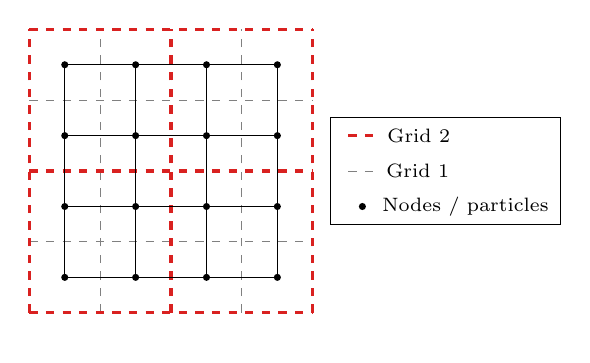
\begin{tikzpicture}[scale=0.9]
  \draw (0,0) --(3,0)--(3,3)--(0,3)--(0,0);
  \draw[white] (0.,0) -- (0,-0.8);
  %%% Grid 1
  \foreach \y in {-0.5,0.5,...,3.5} 
  \draw[dashed,gray] (-0.5,\y) -- (3.5,\y);
  \foreach \x in {-0.5,0.5,...,3.5} 
  \draw[dashed,gray] (\x,-0.5) -- (\x,3.5);
  %%% Grid 2
  \foreach \y in {-0.5,1.5,...,3.5} 
  \draw[dashed,Red,very thick] (-0.5,\y) -- (3.5,\y);
  \foreach \x in {-0.5,1.5,...,3.5} 
  \draw[dashed,Red,very thick] (\x,-0.5) -- (\x,3.5);
  \foreach \y in {0.,1.,...,3.} 
  \foreach \x in {0.,1.,...,3.} 
  \fill (\x,\y) circle(0.05);
  \foreach \y in {0.,1.,...,3.} 
  \draw (0,\y) -- (3.,\y);
  \foreach \x in {0.,1.,...,3.} 
  \draw (\x,0) -- (\x,3);
  \draw (3.75,0.75) rectangle (7.,2.25);
  \fill (4.2,1.) circle (0.05) node [right] {\scriptsize$ \: \: \text{Nodes / particles}$};
  \draw[dashed,gray] (4.,1.5) -- (4.4,1.5) node [right] {\scriptsize$\color{black} \text{Grid 1}$};
  \draw[dashed,very thick,Red] (4.,2.) -- (4.4,2.) node [right] {\scriptsize$\color{black} \text{Grid 2}$};
\end{tikzpicture}


%%% Local Variables:
%%% mode: latex
%%% TeX-master: "../manuscript"
%%% End:
}
  \caption{Geometry, loading and boundary conditions for the tensile impact problem on a two-dimensional elastic medium. The initial velocity is set to $v_d=-200 \: m/s$.}
  \label{fig:PS_domain}
\end{figure}
It is worth noticing that this simulation enables comparisons between the numerical methods in spite of the lack of exact solution for that problem.
Unfortunately, this cannot be circumvented by taking a FEM solution on a very fine mesh as the reference one since, as mentioned in section \ref{sec:plane-strain-problem}, a refinement does not prevent from spurious oscillations and hence, from an overestimation of the plastic strain.



Comparisons of the isovalues of longitudinal PK1 stress $\Pi_{11}$ and cumulated plastic strain $p$ are depicted in figures \ref{subfig:stress_comparison} and \ref{subfig:epls_comparison} respectively for two time steps that correspond to the incident and reflected pressure waves.
The fields are plotted on the current configuration so as to show the deformed shape resulting from each simulation.
Notice that a mesh is reconstructed based on the material points for MPM and DGMPM results for vizualisation purpose.

Before the reflection of the pressure wave, the arising of spurious oscillations arising in MPM and FEM solutions, though much slighter in the latter, and of numerical diffusion in DGMPM(4ppc) one, leads to different assessement of fields.
In addition to the stress peaks occuring in the MPM stress solution in the bottom part of the domain, a checkerboard structure can be seen upstream.
Then, figure \ref{subfig:epls_comparison} shows that the numerical cumulated plastic strains have globally the same shape but different extreme values.

Next, the incident wave reflects on the right end of the solid as a tensile wave so that the bottom part of the boundary starts moving rightward.
After that reflection, similar observations can be made about the MPM and the DGMPM(4ppc) stress solutions, that is, significant oscillations and numerical diffusion respectively.
Moreover, although the FEM and DGMPM(1ppc) stresses are quite similar before the reflection, it is no longer the case after the passage of the tensile wave so that the FEM solution exhibit a maximum that is higher than DGMPM one.
On the other hand, the plastic continues propagating within the domain and no significant difference appears in the numerical cumulated plastic strains.
At that time, it can also be seen that the shapes of the solid domain are quite similar, even though DGMPM solutions leads to a slightly lower vertical displacement of the top left corner of the square.
\begin{figure}[ht]
  \centering
  \subcaptionbox{Stress \label{subfig:stress_comparison}}{\begin{tikzpicture}[scale=1]
  \begin{groupplot}[group style={group size=2 by 4,% columns by rows
      ylabels at=edge left, yticklabels at=edge left,
      horizontal sep=5.ex,
      vertical sep=2ex,},
    enlargelimits=0,
    xmin=0.,xmax=1., ymin=-0.,ymax=1.
    ,axis on top,scale only axis,width=0.18\linewidth
    ,xtick=\empty,ytick=\empty,
    colorbar style={
      title style={
        font=\normalsize,
        at={(1,.5)},
        anchor=north west
      },yticklabel style={font=\normalsize}
      ,at={(current axis.south east)},anchor=south west
    },colormap name=tol
    ]
    %% FIRST ROW (time 1 = 5.10e-4s)
    %%% RANGE -8.6e9 -- 0.57e9
    \nextgroupplot[title={$t=5.10\times 10^{-4} \:s$},ylabel={FEM}]\addplot graphics[xmin=0.,xmax=1., ymin=-0.,ymax=1.] {pngFigures/fem_stress1-crop.png};
    \nextgroupplot[title={$t=1.02\times 10^{-3} \:s$}]\addplot graphics[xmin=0.,xmax=1., ymin=-0.,ymax=1.] {pngFigures/fem_stress2-crop.png};

    \nextgroupplot[ylabel={MPM(1ppc)}]\addplot graphics[xmin=0.,xmax=1., ymin=-0.,ymax=1.] {pngFigures/mpm_stress1-crop.png};
    \nextgroupplot[]\addplot graphics[xmin=0.,xmax=1., ymin=-0.,ymax=1.] {pngFigures/mpm_stress2-crop.png};

    \nextgroupplot[ylabel={DGMPM(1ppc)}]\addplot graphics[xmin=0.,xmax=1., ymin=-0.,ymax=1.] {pngFigures/dgmpm1ppc_stress1-crop.png};
    \nextgroupplot[]\addplot graphics[xmin=0.,xmax=1., ymin=-0.,ymax=1.] {pngFigures/dgmpm1ppc_stress2-crop.png};
    

    \nextgroupplot[ylabel={DGMPM(4ppc)},colorbar horizontal,colorbar  style={
      title style={yshift=-1.5cm},
      title= {$\Pi_{11}\: (GPa)$},
      xtick={-8.6,0.57},
      xticklabels={-8.6,0.57},
    }]
    \addplot[scatter,scatter src=x,mark size=0.pt] coordinates {(-8.6,0.) (0.57,0)};% Fake extreme values to fix scale
    \addplot graphics[xmin=0.,xmax=1., ymin=-0.,ymax=1.] {pngFigures/dgmpm4ppc_stress1-crop.png};
    \nextgroupplot[colorbar horizontal,colorbar  style={
      title style={yshift=-1.5cm},
      title= {$\Pi_{11}\: (GPa)$},
      xtick={-2.3,5.6},
      xticklabels={-2.3,5.6},
    }]
    \addplot[scatter,scatter src=x,mark size=0.pt] coordinates {(-2.3,0.) (5.6,0)};% Fake extreme values to fix scale
    \addplot graphics[xmin=0.,xmax=1., ymin=-0.,ymax=1.] {pngFigures/dgmpm4ppc_stress2-crop.png};
    
  \end{groupplot}
\end{tikzpicture}



%%% Local Variables:
%%% mode: latex
%%% TeX-master: "../manuscript"
%%% End:
}\qquad
  \subcaptionbox{Cumulated plastic strain \label{subfig:epls_comparison}}{\begin{tikzpicture}[scale=1]
  \begin{groupplot}[group style={group size=2 by 4,% columns by rows
      ylabels at=edge left, yticklabels at=edge left,
      horizontal sep=5.ex,
      vertical sep=2ex,},
    enlargelimits=0,
    xmin=0.,xmax=1., ymin=-0.,ymax=1.
    ,axis on top,scale only axis,xtick=\empty,ytick=\empty,width=0.18\linewidth,
    colorbar style={
      title style={
        font=\normalsize,
        at={(1,.5)},
        anchor=north west
      },yticklabel style={font=\normalsize}
      ,at={(current axis.south east)},anchor=south west
    },colormap name=tol]
    %% FIRST ROW (time 1 = 5.10e-4s)
    %%% RANGE -8.6e9 -- 0.57e9
    \nextgroupplot[title={$t=5.10\times 10^{-4} \:s$},ylabel={FEM}]\addplot graphics[xmin=0.,xmax=1., ymin=-0.,ymax=1.] {pngFigures/fem_epeq1-crop.png};
    \nextgroupplot[title={$t=1.02\times 10^{-3} \:s$}]\addplot graphics[xmin=0.,xmax=1., ymin=-0.,ymax=1.] {pngFigures/fem_epeq2-crop.png};

    \nextgroupplot[ylabel={MPM(1ppc)}]\addplot graphics[xmin=0.,xmax=1., ymin=-0.,ymax=1.] {pngFigures/mpm_epeq1-crop.png};
    \nextgroupplot[]\addplot graphics[xmin=0.,xmax=1., ymin=-0.,ymax=1.] {pngFigures/mpm_epeq2-crop.png};

    \nextgroupplot[ylabel={DGMPM(1ppc)}]\addplot graphics[xmin=0.,xmax=1., ymin=-0.,ymax=1.] {pngFigures/dgmpm1ppc_epeq1-crop.png};
    \nextgroupplot[]\addplot graphics[xmin=0.,xmax=1., ymin=-0.,ymax=1.] {pngFigures/dgmpm1ppc_epeq2-crop.png};
    

    \nextgroupplot[ylabel={DGMPM(4ppc)},colorbar horizontal,colorbar  style={
      title style={yshift=-1.5cm},
      title= {$p$},
      xtick={0,.15},
      xticklabels={0,0.15},
    }]
    \addplot[scatter,scatter src=x,mark size=0.pt] coordinates {(0,0.) (0.15,0)};% Fake extreme values to fix scale
    \addplot graphics[xmin=0.,xmax=1., ymin=-0.,ymax=1.] {pngFigures/dgmpm4ppc_epeq1-crop.png};
    \nextgroupplot[colorbar horizontal,colorbar  style={
      title style={yshift=-1.5cm},
      title= {$p$},
      xtick={0.,0.16},
      xticklabels={0,0.16},
    }]
    \addplot[scatter,scatter src=x,mark size=0.pt] coordinates {(0.,0.) (0.16,0)};% Fake extreme values to fix scale
    \addplot graphics[xmin=0.,xmax=1., ymin=-0.,ymax=1.] {pngFigures/dgmpm4ppc_epeq2-crop.png};
    
  \end{groupplot}
\end{tikzpicture}



%%% Local Variables:
%%% mode: latex
%%% TeX-master: "../manuscript"
%%% End:
}
  \caption{Isovalues of the PK1 stress tensor component $\Pi_{11}$ and cumulated plastic strain in a two-dimensional hyperelastic-plastic solids impacting a rigid wall under plane strain. Comparison of FEM (CFL=0.9), MPM (CFL=0.7) and DGMPM solutions using either one particle per cell (CFL=1) or four particles per cell (CFL=0.4).}
  \label{fig:PS_taylor}
\end{figure}

We now propose to look at the above results in more details.
Figures \ref{fig:bottom_line} and \ref{fig:left_line} show the evolution of longitudinal stress and cumulated plastic strain along the bottom and left end of the domain respectively for the same time steps.
First, it can be seen in figure \ref{subfig:bottom1} that the incident wave is described with different level of sharpness by the numerical shemes.
% Note however that no elastic predictor is seen in the stress profiles in contrast to the one-dimensional problem studied above.
Then, the figure also shows the oscillations in the MPM stress solution mentioned above.
Moreover, the superimposition of the stresses resulting from MPM computations using 1ppc or 4ppc shows that refining the particles discretization does not allow removing the numerical noise.
As a consequence, the numerical cumulated plastic strains near the wave front are rather different since the solutions of particle-based methods are ahead of the FEM one.
Upstream that front, the MPM(1ppc) plastic strain exhibits some peaks while this computed with the MPM(4ppc) is closer to the finite element solution.
On the other hand, the two space discretizations lead to DGMPM results that are close from one to another on the plastic plateau.

After the reflection (figure \ref{subfig:bottom2}), the stress profiles are much more different.
The MPM still yields oscillating solutions regardless the space discretization used, and DGMPM results are smoother than the other.
Once Again, the FEM leads to a rather sharp solution.
\begin{figure}[ht]
  \centering
  {\phantomsubcaption{\label{subfig:bottom1}}}
  {\phantomsubcaption{\label{subfig:bottom2}}}
  \begin{tikzpicture}
  \begin{groupplot}[group style={group size=2 by 2, % 3 columns 2 rows
      ylabels at=edge left, yticklabels at=edge left,horizontal sep=2.ex,vertical sep=5.ex,
      xticklabels at=edge bottom,xlabels at=edge bottom},
    ymajorgrids=true,xmajorgrids=true,
    axis on top,scale only axis,width=0.425\linewidth, every x tick scale label/.style={at={(xticklabel* cs:1.05,0.75cm)},anchor=near yticklabel},
    every y tick scale label/.style={at={(yticklabel* cs:1.05,-.9cm)},anchor=near yticklabel}]
    
    %%%%%%%%%%%%%%%%%%%% 
    % ============================== Stress Line
    % t1 
    \nextgroupplot[ylabel=$\Pi_{11} \:(Pa)$,title={(a) $t = 5.10 \times 10^{-4}\: s$},ymin=-1.e10,ymax=7.25e9]
    \addplot[Orange,thick,mark=*,mark repeat=2] table[x=Points:0,y=Piola_Stress:0] {csvFiles/fem_bottom1.csv};
    \addplot[Red,thick,mark=square,only marks] table[x=Points:0,y=Piola:0] {csvFiles/mpm_bottom1.csv};
    \addplot[black!60,thick,mark=o,only marks] table[x=Points:0,y=Piola:0] {csvFiles/mpm4ppc_bottom1.csv};
    \addplot[Blue,thick,mark=asterisk,only marks,mark size=3pt] table[x=Points:0,y=PK1:0] {csvFiles/dgmpm1ppc_bottom1.csv};
    \addplot[Purple,thick,mark=x,only marks,mark size=3pt,mark repeat=2] table[x=Points:0,y=PK1:0] {csvFiles/dgmpm4ppc_bottom1.csv};
    
    % t2 
    \nextgroupplot[title={(b) $t = 1.02 \times 10^{-3}\: s$},ymin=-1.e10,ymax=7.25e9%,ymin=-7.5e9,ymax=100.e9,ytick scale label code/.code={},legend style={at={($(0.75,-0.4)+(0.9cm,0.6cm)$)},legend columns=3}
    ]
    \addplot[Orange,thick,mark=*,mark repeat=2] table[x=Points:0,y=Piola_Stress:0] {csvFiles/fem_bottom2.csv};
    \addplot[Red,thick,mark=square,only marks] table[x=Points:0,y=Piola:0] {csvFiles/mpm_bottom2.csv};
    \addplot[black!60,thick,mark=o,only marks] table[x=Points:0,y=Piola:0] {csvFiles/mpm4ppc_bottom2.csv};
    \addplot[Blue,thick,mark=asterisk,only marks,mark size=3pt] table[x=Points:0,y=PK1:0] {csvFiles/dgmpm1ppc_bottom2.csv};
    \addplot[Purple,thick,mark=x,only marks,mark size=3pt,mark repeat=2] table[x=Points:0,y=PK1:0] {csvFiles/dgmpm4ppc_bottom2.csv};


    % ============================== Cumulated plastic strain Line
    % t1 
    \nextgroupplot[ylabel=$p$,xlabel=$x \: (m)$,ymin=0.,ymax=9.e-2%,ymin=-7.5e9,ymax=100.e9,ytick scale label code/.code={}
    ]
    \addplot[Orange,thick,mark=*,mark repeat=2] table[x=Points:0,y=Equivalent_Plastic_Strain] {csvFiles/fem_bottom1.csv};
    \addplot[Red,thick,mark=square,only marks] table[x=Points:0,y=epeq] {csvFiles/mpm_bottom1.csv};
    \addplot[black!60,thick,mark=o,only marks] table[x=Points:0,y=epeq] {csvFiles/mpm4ppc_bottom1.csv};
    \addplot[Blue,thick,mark=asterisk,only marks,mark size=3pt] table[x=Points:0,y=epeq] {csvFiles/dgmpm1ppc_bottom1.csv};
    \addplot[Purple,thick,mark=x,only marks,mark size=3pt,mark repeat=2] table[x=Points:0,y=epeq] {csvFiles/dgmpm4ppc_bottom1.csv};
    
    % t2
    \nextgroupplot[legend style={at={($(0.75,-0.35)+(0.cm,1cm)$)},legend columns=5},xlabel=$x \: (m)$,ymin=0.,ymax=9.e-2%,ymin=-7.5e9,ymax=100.e9,ytick scale label code/.code={}
    ]
    \addplot[Orange,thick,mark=*,mark repeat=2] table[x=Points:0,y=Equivalent_Plastic_Strain] {csvFiles/fem_bottom2.csv};
    \addplot[black!60,thick,mark=o,only marks] table[x=Points:0,y=epeq] {csvFiles/mpm_bottom2.csv};
    \addplot[Red,thick,mark=square,only marks] table[x=Points:0,y=epeq] {csvFiles/mpm4ppc_bottom2.csv};
    \addplot[Blue,thick,mark=asterisk,only marks,mark size=3pt] table[x=Points:0,y=epeq] {csvFiles/dgmpm1ppc_bottom2.csv};
    \addplot[Purple,thick,mark=x,only marks,mark size=3pt,mark repeat=2] table[x=Points:0,y=epeq] {csvFiles/dgmpm4ppc_bottom2.csv};

    \addlegendentry{fem \:}
    \addlegendentry{mpm (1ppc) \:}
    \addlegendentry{mpm (4ppc) \:}
    \addlegendentry{dgmpm (1ppc) \:}
    \addlegendentry{dgmpm (4ppc) \:}
    
    
  \end{groupplot}
\end{tikzpicture}



%%% Local Variables:
%%% mode: latex
%%% TeX-master: "../manuscript"
%%% End:

  \caption{Comparison of the longitudinal stress component and cumulated plastic strain along the bottom boundary of the domain at two times.}
  \label{fig:bottom_line}
\end{figure}
Furthermore, the MPM cumulated plastic strain curves oscillate around the FEM one which, in turn, is above these computed with the DGMPM.

The above observations are even more significant when looking at the evolution of fields along the left end of the square (figure \ref{fig:left_line}).
In figure \ref{subfig:left1}, FEM and DGMPM stress profiles show good agreement while spurious oscillations pollute MPM ones. 
Although FEM and DGMPM stresses are similar, it is not the case for the cumulated plastic strains for which the numerical results differ more.
Thus, the MPM yields the highest values of cumulated plastic strain at the top left corner of the domain.
The results depicted at the subsequent time show tremendous oscillations in the MPM(1ppc) solution for which the longitudinal stress varies roughly from $-7 \: GPa$ to $1 \: GPa$ in the bottom part of the left boundary.
These oscillations are reduced, though not completely removed, in the MPM(4ppc) results. 
On the other hand, DGMPM and FEM solutions no longer fit.
\begin{figure}[ht]
  \centering
  {\phantomsubcaption{\label{subfig:left1}}}
  {\phantomsubcaption{\label{subfig:left2}}}
  \input{pgfFigures/left_line}
  \caption{Comparison of the longitudinal stress component and cumulated plastic strain along the left boundary of the domain at two times.}
  \label{fig:left_line}
\end{figure}
It appears that the stress curve corresponding to the latter is bounded by these of the DGMPM(4ppc) and DGMPM(1ppc), the lower bound being given by the single particle space discretization.
At last, the cumulated plastic strain curves show similar behaviors to those of the previous time step except close to the bottom left corner of the domain.
In that region, the plastic flow developed differently depending on the numerical solution considered.
Both DGMPM curves are below that computed with the FEM while the profiles resulting from MPM computations are less regular than the other.

\subsection{Non-linear hardening material}
\label{sec:non-linear-hardening}
Reprendre le cas test hyperelastique de la these?


%%% Local Variables:
%%% mode: latex
%%% TeX-master: "manuscript"
%%% End:



\section{Conclusion}
\label{sec:conclusion}
\subsection{Summary of the chapter}

In this chapter, the characteristic structure of the solution of hyperbolic problems in elastic-plastic solids in two space dimensions has been highlighted.
It is known since the 50s that plastic flow in two-dimensional solids yields two families of waves whose speeds depend on the stress state, the slow and fast waves.
In addition, these plastic waves may have an impact on all stress components in contrast to elastic discontinuities, hence the name of combined-stress waves.
During the 60s, attention has been paid to simple waves in particular two-dimensional problems thus providing, among others, solutions of Picard problems in an elastic-plastic medium undergoing step loadings \cite{Clifton,Ting68,Ting73}.
% Idem pour ting ? c'est dit dans l'intro ? voir ce qui est fait dans le 73
The singular nature of such problems lies in the fact that the characteristic structure of the solution depends on the external loading undergone.
Indeed, it has been shown \cite{Clifton} that boundary conditions can lead to plastic flow involving one fast, one slow, or both simple waves.
Therefore, it is crucial to be able to identify typical stress paths followed in each simple wave in order to link the initial data to a given stress state, and subsequently to determine the occurring wave pattern.

%Besides these works, investigations on plastic shocks have been carried out.
%The existence of such solutions is due to the state law for the hydrostatic pressure which dominates deviatoric effects.


$\newline$
%% Lin et Ballman
Based on these works, an iterative Riemann solver \cite{Lin_et_Ballman}, whose procedure has been recalled in section \ref{sec:stress_paths_num}, has been developed for the numerical solution of the thin-walled tube problem. 
This solver relies on the ability to connect a stationary state to initial data by a characteristic wave pattern.
% L'idée ici c'est de généraliser cette approche pour tous les problèmes 2D
Following this approach, identifying characteristic wave patterns for general elastoplastic problems in two space dimensions should allow to enrich the numerical solution with the knowledge of physics.
For that purpose, the characteristic analysis of two-dimensional problems in elastic-plastic materials with linear isotropic hardening under plane strain and plane stress, in projection in an arbitrary direction of space, has been carried out in section \ref{sec:charac_plast}.
Fast and slow waves are also involved in the solution so that applying the method of characteristic through the simple waves provides a system of ODEs.
Integration of this system leads to integral curves in terms of velocity and stress components that are followed inside the combined-stress waves.
%Integration of this system leads to combined stress paths that are followed between initial and final stress states on the one hand, and to the integral curves in terms of velocity components involving integral along those loading paths on the other hand.
Specializing the ODEs to one direction of a Cartesian grid, it has been shown in section \ref{sec:stress_paths} that the loading paths satisfied through slow and fast waves are perpendicular in the stress space for both plane strain and plane stress.
Moreover, it has been established that the stress paths exhibit particular behavior in the space $(\sigma_{11},\sigma_{22},\sigma_{12})$, that is $d\sigma_{11}=0$, $d\sigma_{12}=0$ or $d\sigma_{22}=0$, for special values of the components of the acoustic tensor.
These situations are achieved for different stress states depending on whether the problem involves plane stresses of plane strains as shown in section \ref{sec:stress_paths}.

$\newline$
The complexity of the ODEs derived in section \ref{sec:charac_plast} prevents identifying all the singularities which may occur along the loading paths.
Hence, the mathematical analysis has been supplemented with numerical results consisting of the integration of stress paths from arbitrary initial stress values lying on the initial yield surface, for the particular direction $\vect{e}_1$.

%% Thin-walled tube
First, in section \ref{sec:num_thin-walled} the loading paths resulting from the integration of the ODEs derived in section \ref{sec:charac_plast} have been compared to those of Clifton \cite{Clifton}.
The two different formulations, respectively based on elastoplastic stiffnesses and softnesses, show  good agreement.

%% Cont. planes
Second, the evolution of stress components across fast and slow waves under plane stress has been looked at in section \ref{sec:num_plane_stress}.
It appears that though the loading paths are rather complex in stress space through a fast wave, the stress evolution in the deviatoric plane is restricted to the initial yield surface until one direction of pure shear is reached.
A singularity then occurs so that the numerical integration cannot be pursued.
On the other hand, the loading paths resulting from the integration of ODEs satisfied inside a slow wave exhibit complex shapes along which $\sigma_{11}$ varies much less than the other stress components.

%% Def. planes
Third, the plane strain case has been considered in section \ref{sec:num_plane_strain}.
Once again, the integral curves inside a fast wave show complex shapes in stress space, and an evolution restricted to the initial yield surface in the deviatoric plane.
In that case, however, the paths may follow a direction of pure tension/compression in the latter plane so that the plastic flow is radial for high values of the hardening modulus. 
In contrast, the paths inside slow waves first rotate on the yield surface and then lead to a stress state of pure shear in the deviatoric plane.

\subsection{Towards a two-dimensional elastoplastic Riemann solver}
The physical structures emphasized in this chapter enable a better understanding of the propagation of waves in two-dimensional elastoplastic media, although further investigations are required.
On the other hand, the loading paths followed in fast and slow simple waves can be used in order to improve the numerical simulation of these problems.

%% Lin et Ballman
One possibility is to generalize the approach proposed by Lin and Ballman \cite{Lin_et_Ballman} based on the clues provided above.
The idea would be to successively assume stationary states of the Riemann problem in terms of stress $\sigma_{11}$, $\sigma_{12}$ and $\sigma_{22}$ in order to build stress paths starting from the initial data.
Namely, considering the direction $\vect{e}_1$, the loading paths followed through a slow wave can be integrated backward starting from the guessed state.
Then, different situations may occur:
\begin{itemize}
\item[(1-a)] the curve thus obtained crosses the initial yield surface at a point where $\sigma_{22}$ satisfies the initial data.
  In that case, the elastic discontinuities led to that stress state so that the characteristic structure corresponds to that depicted in figure \ref{fig:charac}\subref{subfig:charac1}.
\item[(1-b)] if on the other hand the point reached on the initial yield does not satisfy the initial stress $\sigma_{22}$, a fast wave is added in order to browse the initial yield surface until the initial data is recovered.
  This situation is depicted in figure \ref{fig:charac}\subref{subfig:charac2}.
\item[(2-a)] the curve resulting from the reverse integration across a slow wave intersects the plane $\sigma_{12}=0$.
  Then, assuming that the paths of slow waves are symmetric with respect to that plane, a fast wave is added in order to reach the initial yield surface at the initial value of $\sigma_{22}$.
  Indeed, the fast waves have been shown to yield horizontal paths in the ($\sigma_{11},\sigma_{12}$) plane, in such a way that only that type of wave enables the achievement of the initial elastic domain.
  This also corresponds to figure \ref{fig:charac}\subref{subfig:charac2}.
\item[(2-b)] if at last, the guessed state is such that $\sigma_{12}=0$, a fast wave allows reaching the initial yield surface as depicted in figure \ref{fig:charac}\subref{subfig:charac3}.
\end{itemize}

\begin{figure}[h!]
  \centering
  \subcaptionbox{One slow wave \label{subfig:charac1}}{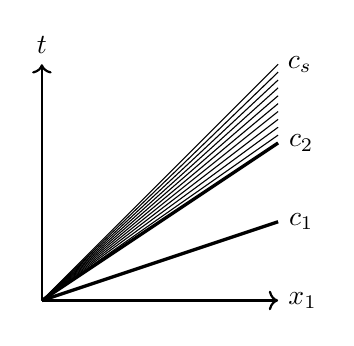
\begin{tikzpicture}
    \draw[thick, ->] (0,0) -- (3.,0) node [right] {$x_1$};
    \draw[thick, ->] (0,0) -- (0,3) node [above] {$t$};
    \draw[very thick] (0,0) -- (3,1) node [right] {$c_1$};
    \draw[very thick] (0,0) -- (3,2) node [right] {$c_2$};
    \foreach \x in {0.1,0.2,...,0.9}
    \draw (0,0) -- (3,2+\x);
    \draw (0,0) -- (3,3) node [right] {$c_s$};
\end{tikzpicture}} \qquad 
  \subcaptionbox{Both simple waves \label{subfig:charac2}}{\input{pgfFigures/charac_structuresSlFa}} \qquad 
  \subcaptionbox{One fast wave \label{subfig:charac3}}{\input{pgfFigures/charac_structuresFa}}
  \caption{Characteristic structures possibly occurring in two-dimensional elastic-plastic solids.}
  \label{fig:charac}
\end{figure}
Notice however that the above elementary loading paths are based on strong assumptions about the symmetry of the loading paths that have not been shown so far.
As a result, additional work must be performed in order to develop this approach and to introduce it in numerical methods.
Moreover, the hardening of the material may modify the behavior of the loading paths and have not been considered yet.
At last, the generalization of the approach followed in this chapter to more complex hardening models (kinematic, nonlinear etc.) and other yield surfaces would be very interesting for the understanding of the physics. 

%%% Local Variables:
%%% mode: latex
%%% TeX-master: "manuscript"
%%% End:



\bibliographystyle{elsarticle-num}
\bibliography{Biblio}


\end{document}
\endinput


%%% Local Variables:
%%% mode: latex
%%% TeX-master: t
%%% End:
